\chapter{GSM}
\section{Interfaces}
\label{sec:interfaces}
The following table contains a brief description of the interfaces used inside a GSM network.
On the upper part the interfaces for the Network Subsystem are listed and on the lower part the interfaces for the Base Station Subsystem can be found.

\begin{table}[h!]
\centering
\begin{tabular}{lll}
\toprule
Name			&Between					&Function\\
\midrule
$A$				&MSC $\leftrightarrow$ BSS	&BSS management data for Mobility Management\\
				&							&and Call Control\\
$B$				&MSC $\leftrightarrow$ VLR	&MSC receives data about MSs in the current area\\
				&							& and sends data from Location Updates\\
$C$				&MSC $\leftrightarrow$ HLR	&MSC can request routing data during call setup\\
				&							&and send \eg charging information\\
$D$				&HLR $\leftrightarrow$ VLR	&Exchange of location-dependent subscriber data\\
				&							&and updating the HLR (MSRN \etc)\\
$E$				&MSC $\leftrightarrow$ MSC	&Executing a Handover when subscriber changes\\
				&							&to a new MSC\\
$F$				&MSC $\leftrightarrow$ EIR	&Checking white-/grey- and blacklists before\\
				&							&giving access to the network\\
$G$				&VLR $\leftrightarrow$ VLR	&Connects VLR of different MSCs to exchange\\
				&							&subscriber data during a handover\\
\midrule
$A_\text{bis}$	&BSC $\leftrightarrow$ BTS	&BSC receives data from MS via the BTS\\
$U_m$			&BTS $\leftrightarrow$ MS	&Registration procedure, call data \etc as well\\
				&							&as broadcast information about the network\\
				&							&and the base station\\
\bottomrule
\end{tabular}
\caption{Interface found in the GSM network.}
\end{table}

\newpage
\section{Channel Combinations}
\label{sec:combinations}
The following table contains the possible combinations of channels inside the different Multiframes.
The respective frame type is also indicated in the lower part of the table.
\begin{table}[h!]
\centering
\begin{tabular}{lccccccccc}
\toprule
					&M1&M2&M3&M4&M5&M6&M7&M8&M9\\
\midrule
TCH/F				&\cellcolor[gray]{0.7}&&&&&&&\cellcolor[gray]{0.7}&\cellcolor[gray]{0.7}\\
TCH/H				&&\cellcolor[gray]{0.7}&\cellcolor[gray]{0.7}&&&&&&\\
TCH/H				&&&\cellcolor[gray]{0.7}&&&&&&\\
BCCH				&&&&\cellcolor[gray]{0.7}&\cellcolor[gray]{0.7}&\cellcolor[gray]{0.7}&&&\\
FCCH				&&&&\cellcolor[gray]{0.7}&\cellcolor[gray]{0.7}&&&&\\
SCH					&&&&\cellcolor[gray]{0.7}&\cellcolor[gray]{0.7}&&&&\\
CCCH				&&&&\cellcolor[gray]{0.7}&\cellcolor[gray]{0.7}&\cellcolor[gray]{0.7}&&&\\
SDCCH				&&&&&\cellcolor[gray]{0.7}&&\cellcolor[gray]{0.7}&&\\
SACCH				&\cellcolor[gray]{0.7}&\cellcolor[gray]{0.7}&\cellcolor[gray]{0.7}&&\cellcolor[gray]{0.7}&&\cellcolor[gray]{0.7}&\cellcolor[gray]{0.7}&\cellcolor[gray]{0.7}\\
FACCH				&\cellcolor[gray]{0.7}&\cellcolor[gray]{0.7}&\cellcolor[gray]{0.7}&&&&&\cellcolor[gray]{0.7}&\\
\midrule
Multiframe Type		&26&26&26&51&51&51&51&26&26\\
\bottomrule
\end{tabular}
\caption{Possible mappings of channels onto Multiframes}
\end{table}


\chapter{OsmocomBB}
This section contains general information about how to operate and setup the OsmocomBB framework and the Motorola C123.
\section{Installation}
\label{sec:osmo_install}
The environment used for this project was a Thinkpad X220 Tablet running Xubuntu Linux 11.10.
The instructions should work for any other distribution of the Ubuntu product palette.

\begin{enumerate}
	\item Build libraries must be installed on the operating system to enable compiling libraries.
	\begin{lstlisting}
sudo apt-get install libtool shtool autoconf git-core 
pkg-config make gcc wget
	\end{lstlisting}
	\item The GNU Arm cross compiler toolchain needs to be installed so the firmware for the Motorola C123 can be built.
	It will be added as a repository to \texttt{sources} so it can be easily removed if it is not required any more.
	\begin{lstlisting}
sudo add-apt-repository ppa:bdrung/bsprak
sudo apt-get update
sudo apt-get install arm-elf-toolchain
	\end{lstlisting}
	\item The source code needs to be obtained.
	This can be either done by checking out the latest version of the framework from the developers, or by using the code on the CD.
	\begin{lstlisting}
git clone git://git.osmocom.org/osmocom-bb.git
	\end{lstlisting}
	\item At this point some firmwares had build errors, therefore we will compile only the firmware for the Calypso board used by the Motorola C123.
	This constraint might not be necessary if a newer version of the framework is used.
	In the \texttt{src} directory of the OsmocomBB framework the build process can be started.
	\begin{lstlisting}
make BOARDS=compal_e88
	\end{lstlisting}
	\item If a new version of OsmocomBB is used, the extra code from this project must be included in the build.
	The two files \texttt{catcher.c} and \texttt{app\_catcher.c} must be moved to \texttt{osmocom-bb/src/host/layer23/src/misc} and the \texttt{Makefile.am} must be edited to include the new code.
	\begin{lstlisting}
bin_PROGRAMS = bcch_scan ... cbch_sniff catcher
catcher_SOURCES = ../common/main.c app_catcher.c
	\end{lstlisting}
\end{enumerate}

\section{Usage}
\label{sec:osmo_usage}
To use a program written in the framework, the Motorola C123 needs to be flashed with the custom firmware.
This can be done with the \texttt{osmocon} application. 
\begin{lstlisting}
cd src/host/osmocon
sudo ./osmocon -p /dev/ttyUSB0 -m c123xor
 ../../target/firmware/board/compal_e88/layer1.compalram.bin
\end{lstlisting}
After \texttt{osmocon} is started and running any application can be started with root privileges.
\begin{lstlisting}
cd ../layer23/src/misc/
sudo catcher
\end{lstlisting}
\newpage
\section{Serial Cable Schematics}
\label{sec:osmo_serial_schematics}
A T191 unlock cable used to connect the Motorola C123 can either be obtained by ordering it from one of the mentioned stores or by building it from scratch.
These are the schematics required for building the unlock cable.
\vfill
\begin{center}
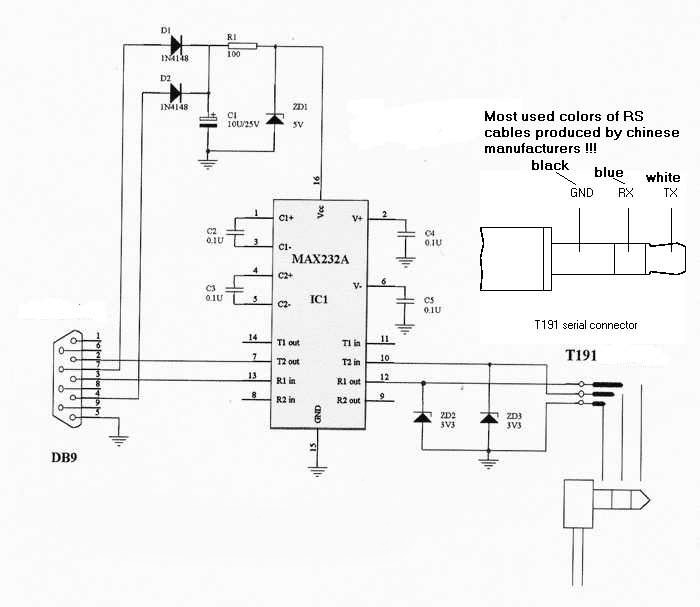
\includegraphics[width=.9\textwidth]{../Images/t191cable}
\end{center}
\vfill
\chapter{IMSI Catcher Detection System}
This section will cover some code related topics of the ICDS.
\section{Extextions}
\label{sec:extensions}
Rules, evaluators and filters are implemented in a way that new modules can be added quickly by way of inheritance and instantiating them in the constructor of the controller so they are known to the system.
The following example shows how to implement a new rule and add it to the system.
This exemplary process is nearly the same for filters and evaluators.

At first this base class has to be derived.
\begin{lstlisting}
class Rule:
    #set whether the rule should be used by the 
    #controller
    is_active = False
    #string that will identify the rule in the report
    identifier = 'Rule'

    #the logic of the rule, will be called by controller
    def check(self, arfcn, base_station_list):
        return RuleResult.CRITICAL
\end{lstlisting}

The new rule class needs to override the check method to do something meaningful.
The identifier should also be set to a proper value.
\begin{lstlisting}
class MyRule (Rule):
    identifier = 'My own Rule'
    def check(self,arfcn, base_station_list):
        result = RuleResult.CRITICAL
        #do some logic here and set result 
        return result
\end{lstlisting}
\texttt{arfcn} and \texttt{base\_station\_list} are given to the check method by the controller.
The first parameter is the ARFCN of the base station to which the evaluation will be applied.
The second one is a list of all the base stations with complete information as far as it has been
obtained by the ICDS.

After it has been implemented it can be instatiated and added to the list of active rules in the 
constructor of the controller.
\begin{lstlisting}
class PyCatcherController:
    ...
    def __init__ (self):
        ...
        self.my_rule = MyRule()
        self.my_rule.is_active = True
        self._rules.add(self._my_rule)
        ...
\end{lstlisting}
\section{Example Configuration}
\label{sec:example_config}
This example configuration has been used for the evaluation in the Freiburg area.
\begin{lstlisting}
#Core Configuration ---------------------------------------

#Settings for the Motorola C123 .
Device_settings = { 'mobile_device' : '/dev/ttyUSB0',
                    'xor_type' : 'c123xor',
                    'firmware' : 'compal_e88',
                   }

#Location of the osmocom library.
Osmocon_lib = '''/home/tom/imsi-catcher-detection/Src/
osmolib/src'''

#Generates commands from location and device settings.
#Does normally not have to be edited.
Commands = {'osmocon_command' : [Osmocon_lib + 
    '/host/osmocon/osmocon', 
    '-p', Device_settings['mobile_device'], 
    '-m', Device_settings['xor_type'], 
    Osmocon_lib + '/target/firmware/board/' 
    + Device_settings['firmware']
    + '/layer1.compalram.bin'],
    'scan_command' : [Osmocon_lib 
    + '/host/layer23/src/misc/catcher'],
}

#Rules Configuration --------------------------------------

#A list of providers that should be taken as legitimate.
Provider_list = ['T-Mobile', 'O2', 'Vodafone', 'E-Plus']

#Countries where the given providers have presence.
Provider_Country_list = {
    'T-Mobile':'Germany',
    'O2':'Germany',
    'Vodafone':'Germany',
    'E-Plus':'Germany'
}

#Comma separated list of LACs that can be observed in the
#given area.
LAC_mapping = {
    'T-Mobile' : [21014,21015],
    'O2' : [50945],
    'Vodafone' : [793],
    'E-Plus' : [138,588]
}

#Frequency intervals that are registered to the 
#given providers.
ARFCN_mapping = {
    'T-Mobile' : [(13,39),(81, 102),(122,124),(587,611)],
    'O2' : [(0,0),(1000,1023),(637,723)],
    'Vodafone' : [(1,12),(50,80),(103,121),(725,751)],
    'E-Plus' : [(975,999),(777,863)]
}

#How much % the LAC of a base station can deviate from the
#median before throwing an error (range 0 to 1 where 0 
#means no tolerance).
LAC_threshold = 0

#How much % the rx level is allowed to be away from the
#interval located in the Location Area Database
DB_RX_threshold = 0.05

#How much % the rx is allowed to change during the course
#of a scan.
CH_RX_threshold = 0.02

#Database Configuration -----------------------------------

#The API key for OpenCellID.
#Can be freely obtained by registering on the web site. 
Open_Cell_ID_Key = 'd7a5bc3f21b44d4bf93d1ec2b3f83dc4'

#Path to the folder where databases should be saved to or
#loaded from. The ICDS will look in this folder if databa-
#ses are available.
Database_path = '''/home/tom/imsi-catcher-detection/Src
/PyCatcher/Databases/'''
\end{lstlisting}

\chapter{System Information}
\label{sec:system_infos}
The following pages contain parsed System Information Messages of type 1-4  for reference.
\begin{figure}
\centering
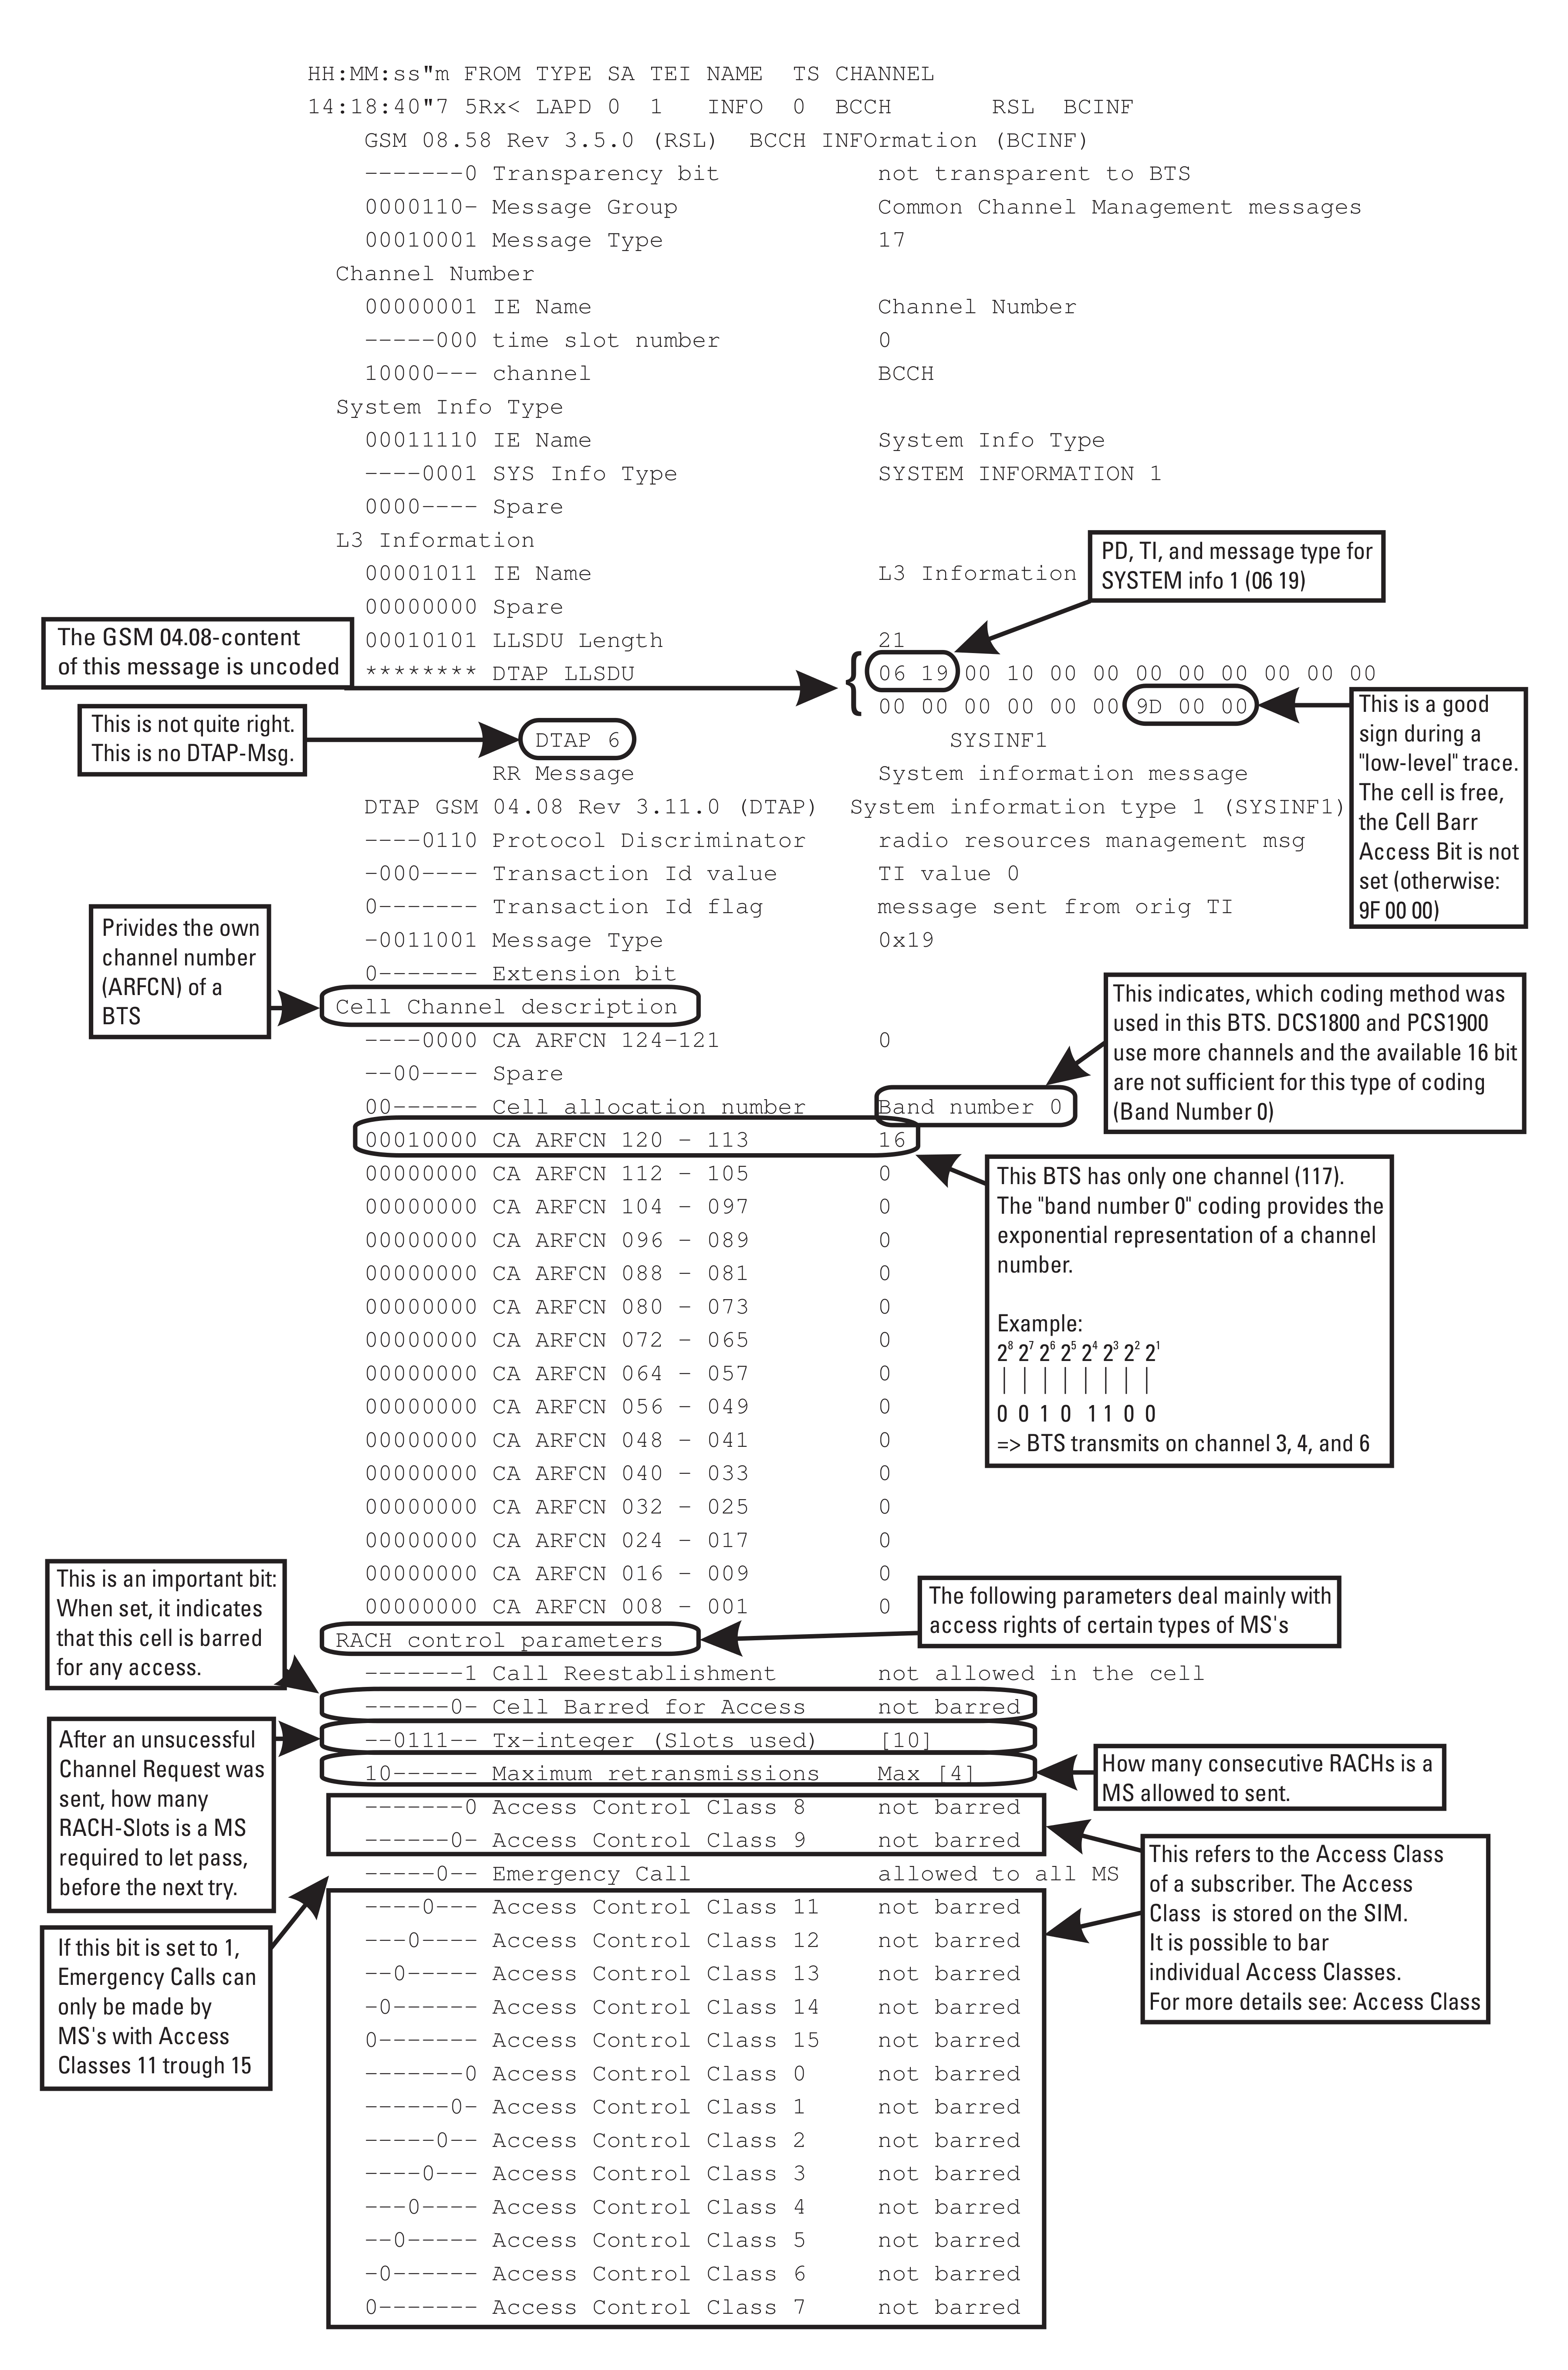
\includegraphics[width=.9\textwidth]{../Images/sysinfo1}
\caption{System Information 1 Message}
\end{figure}
\begin{figure}
\centering
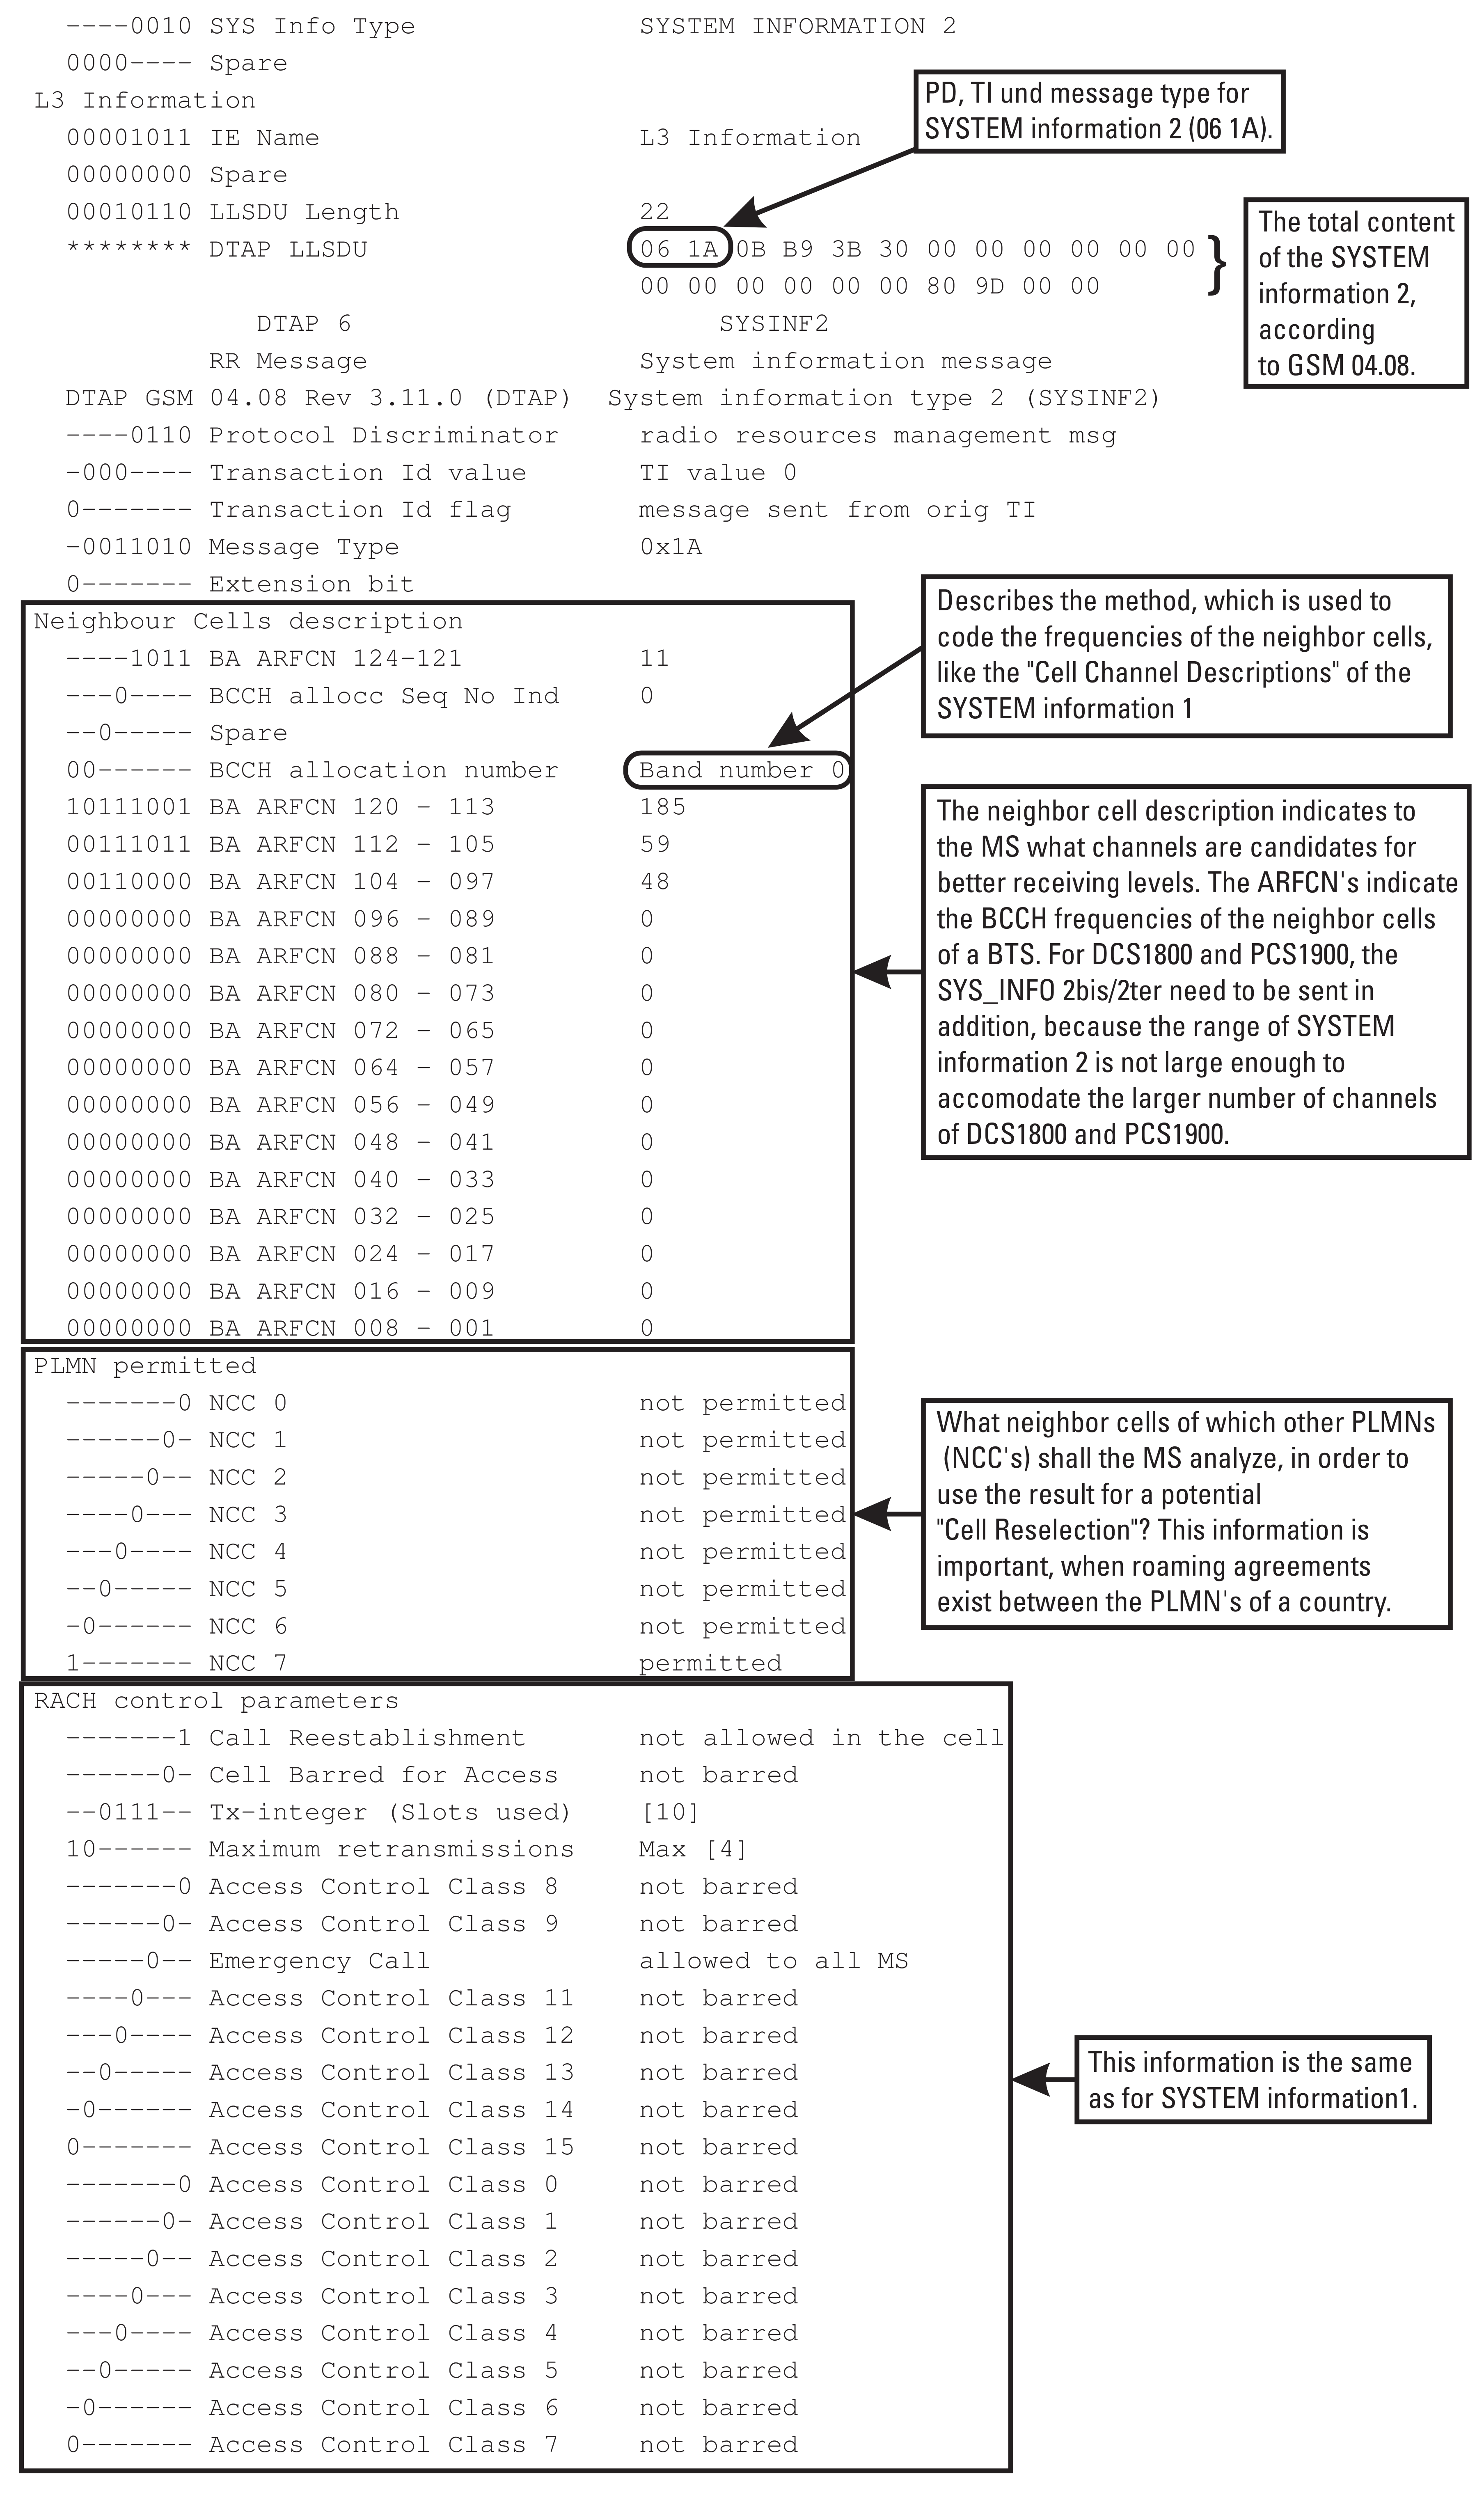
\includegraphics[width=.9\textwidth]{../Images/sysinfo2}
\caption{System Information 2 Message}
\end{figure}
\begin{figure}
\centering
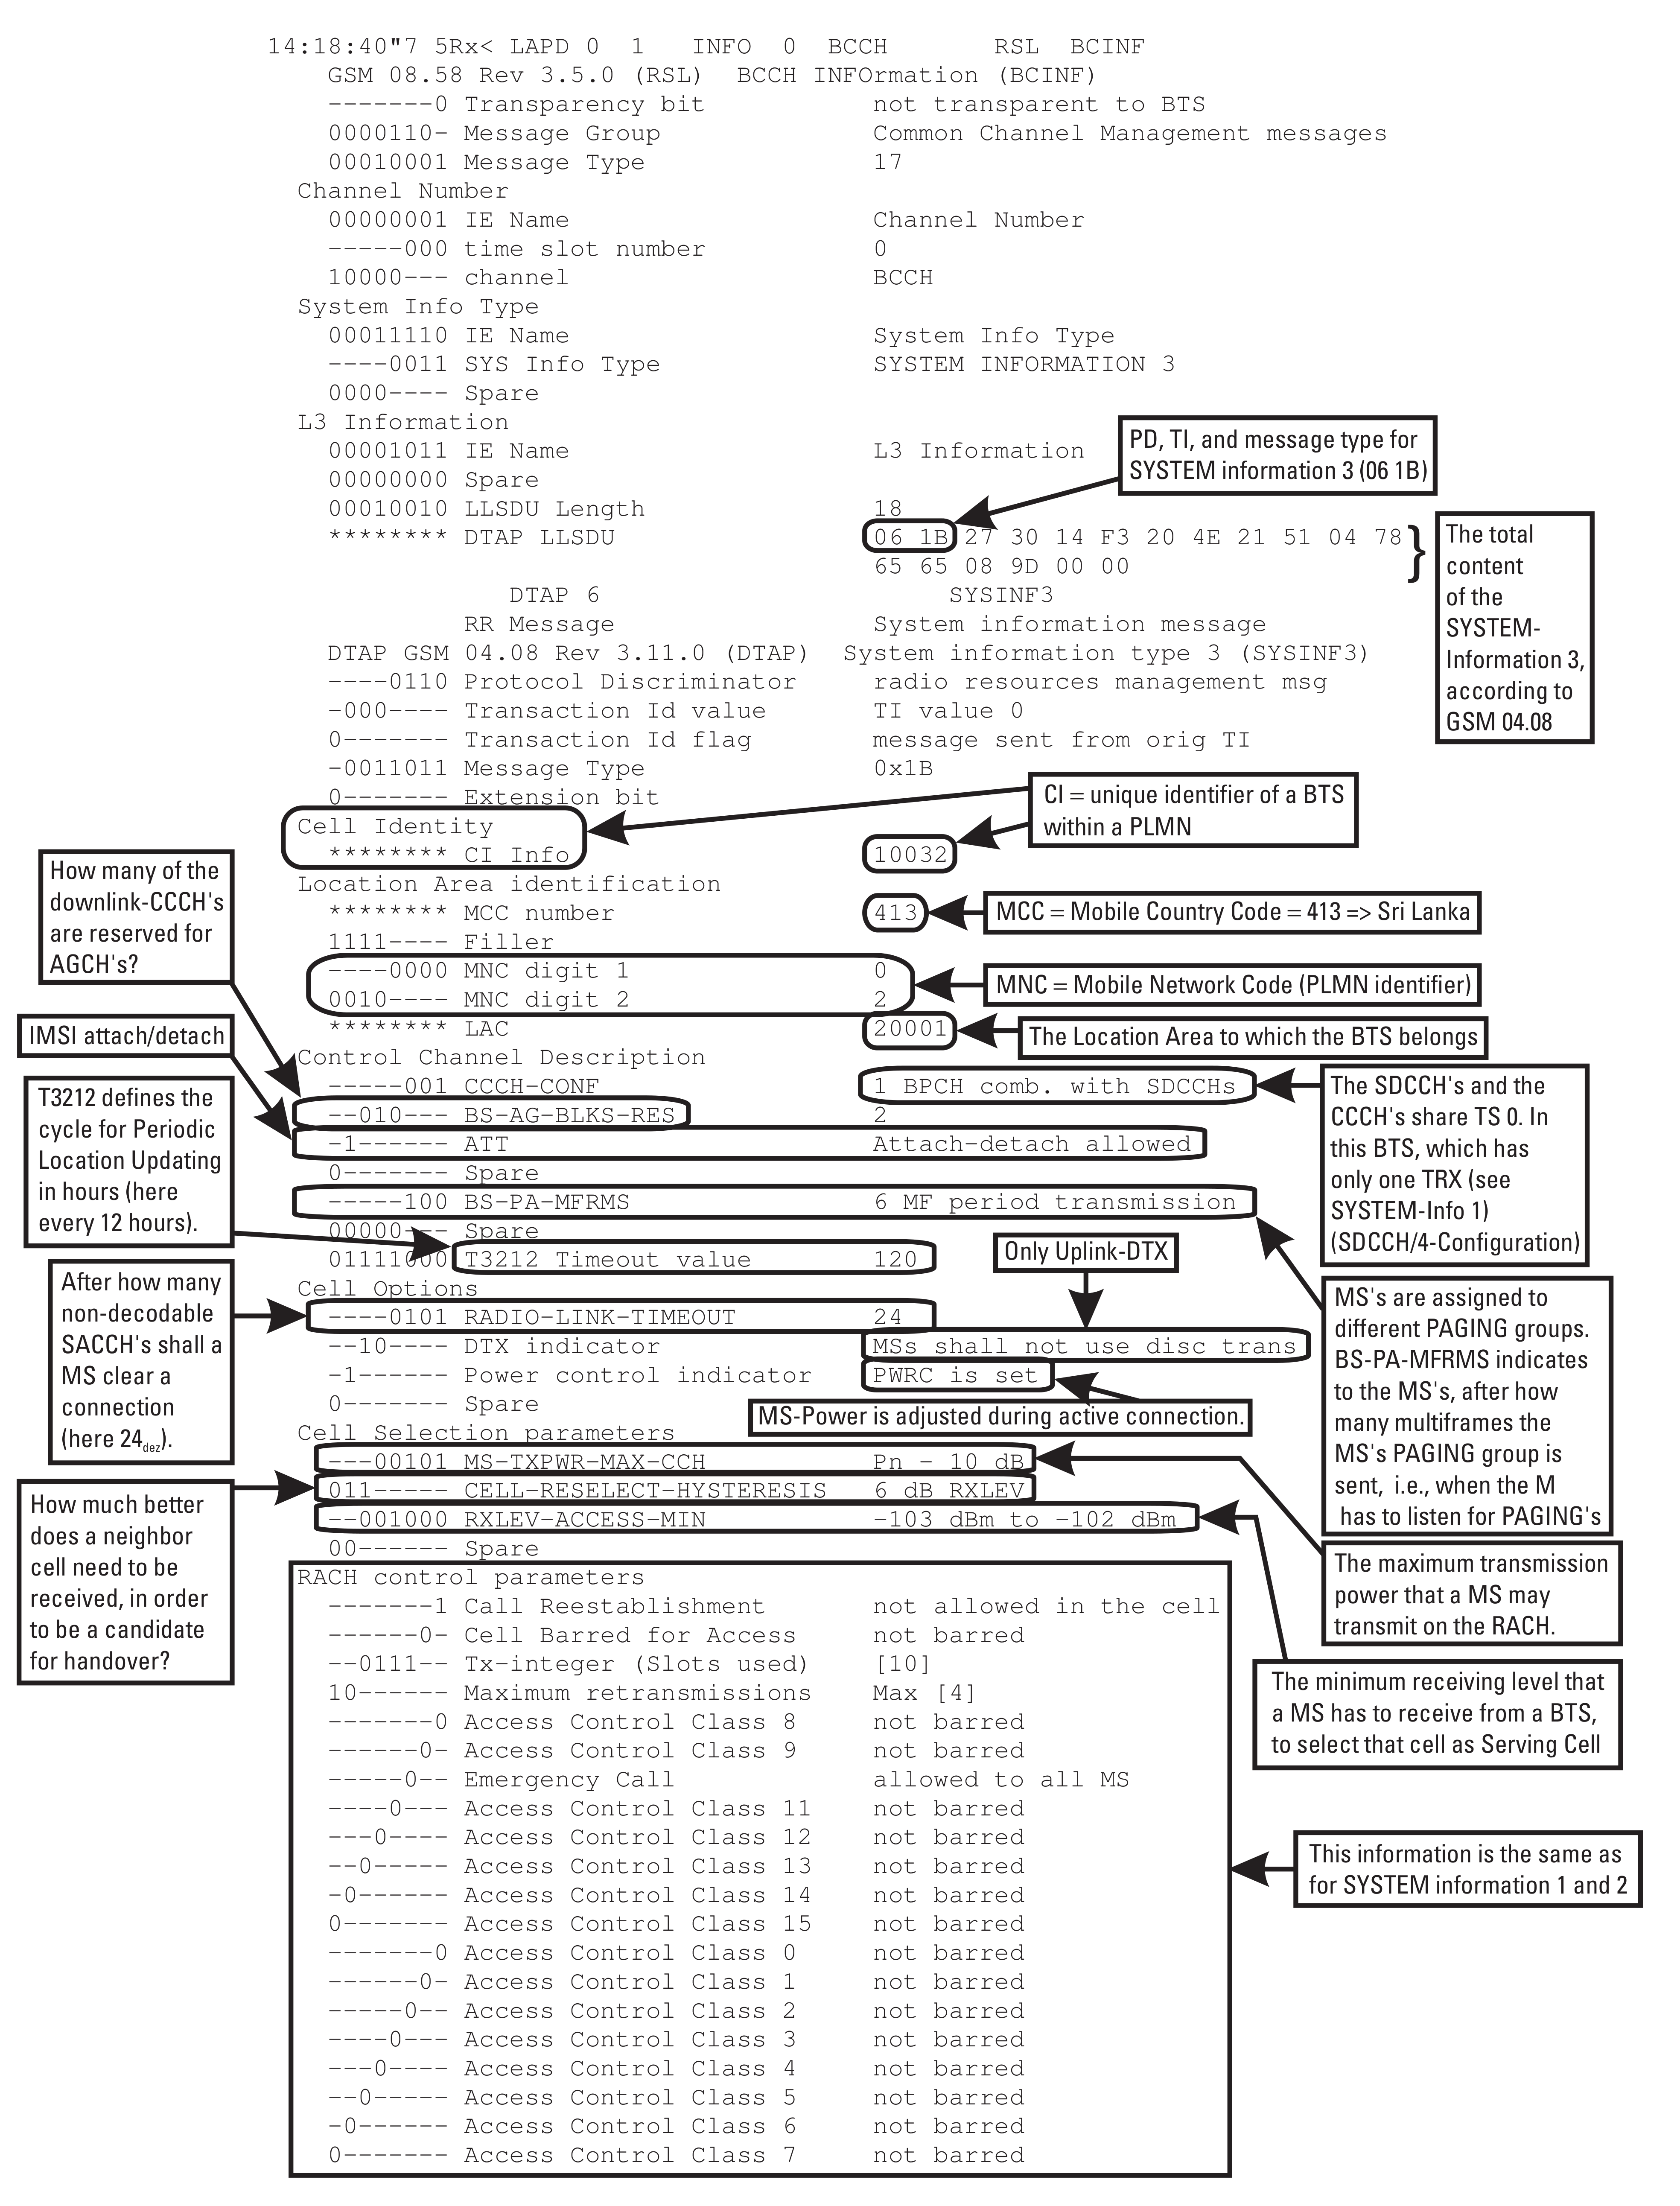
\includegraphics[width=.9\textwidth]{../Images/sysinfo3}
\caption{System Information 3 Message}
\end{figure}
\begin{figure}
\centering
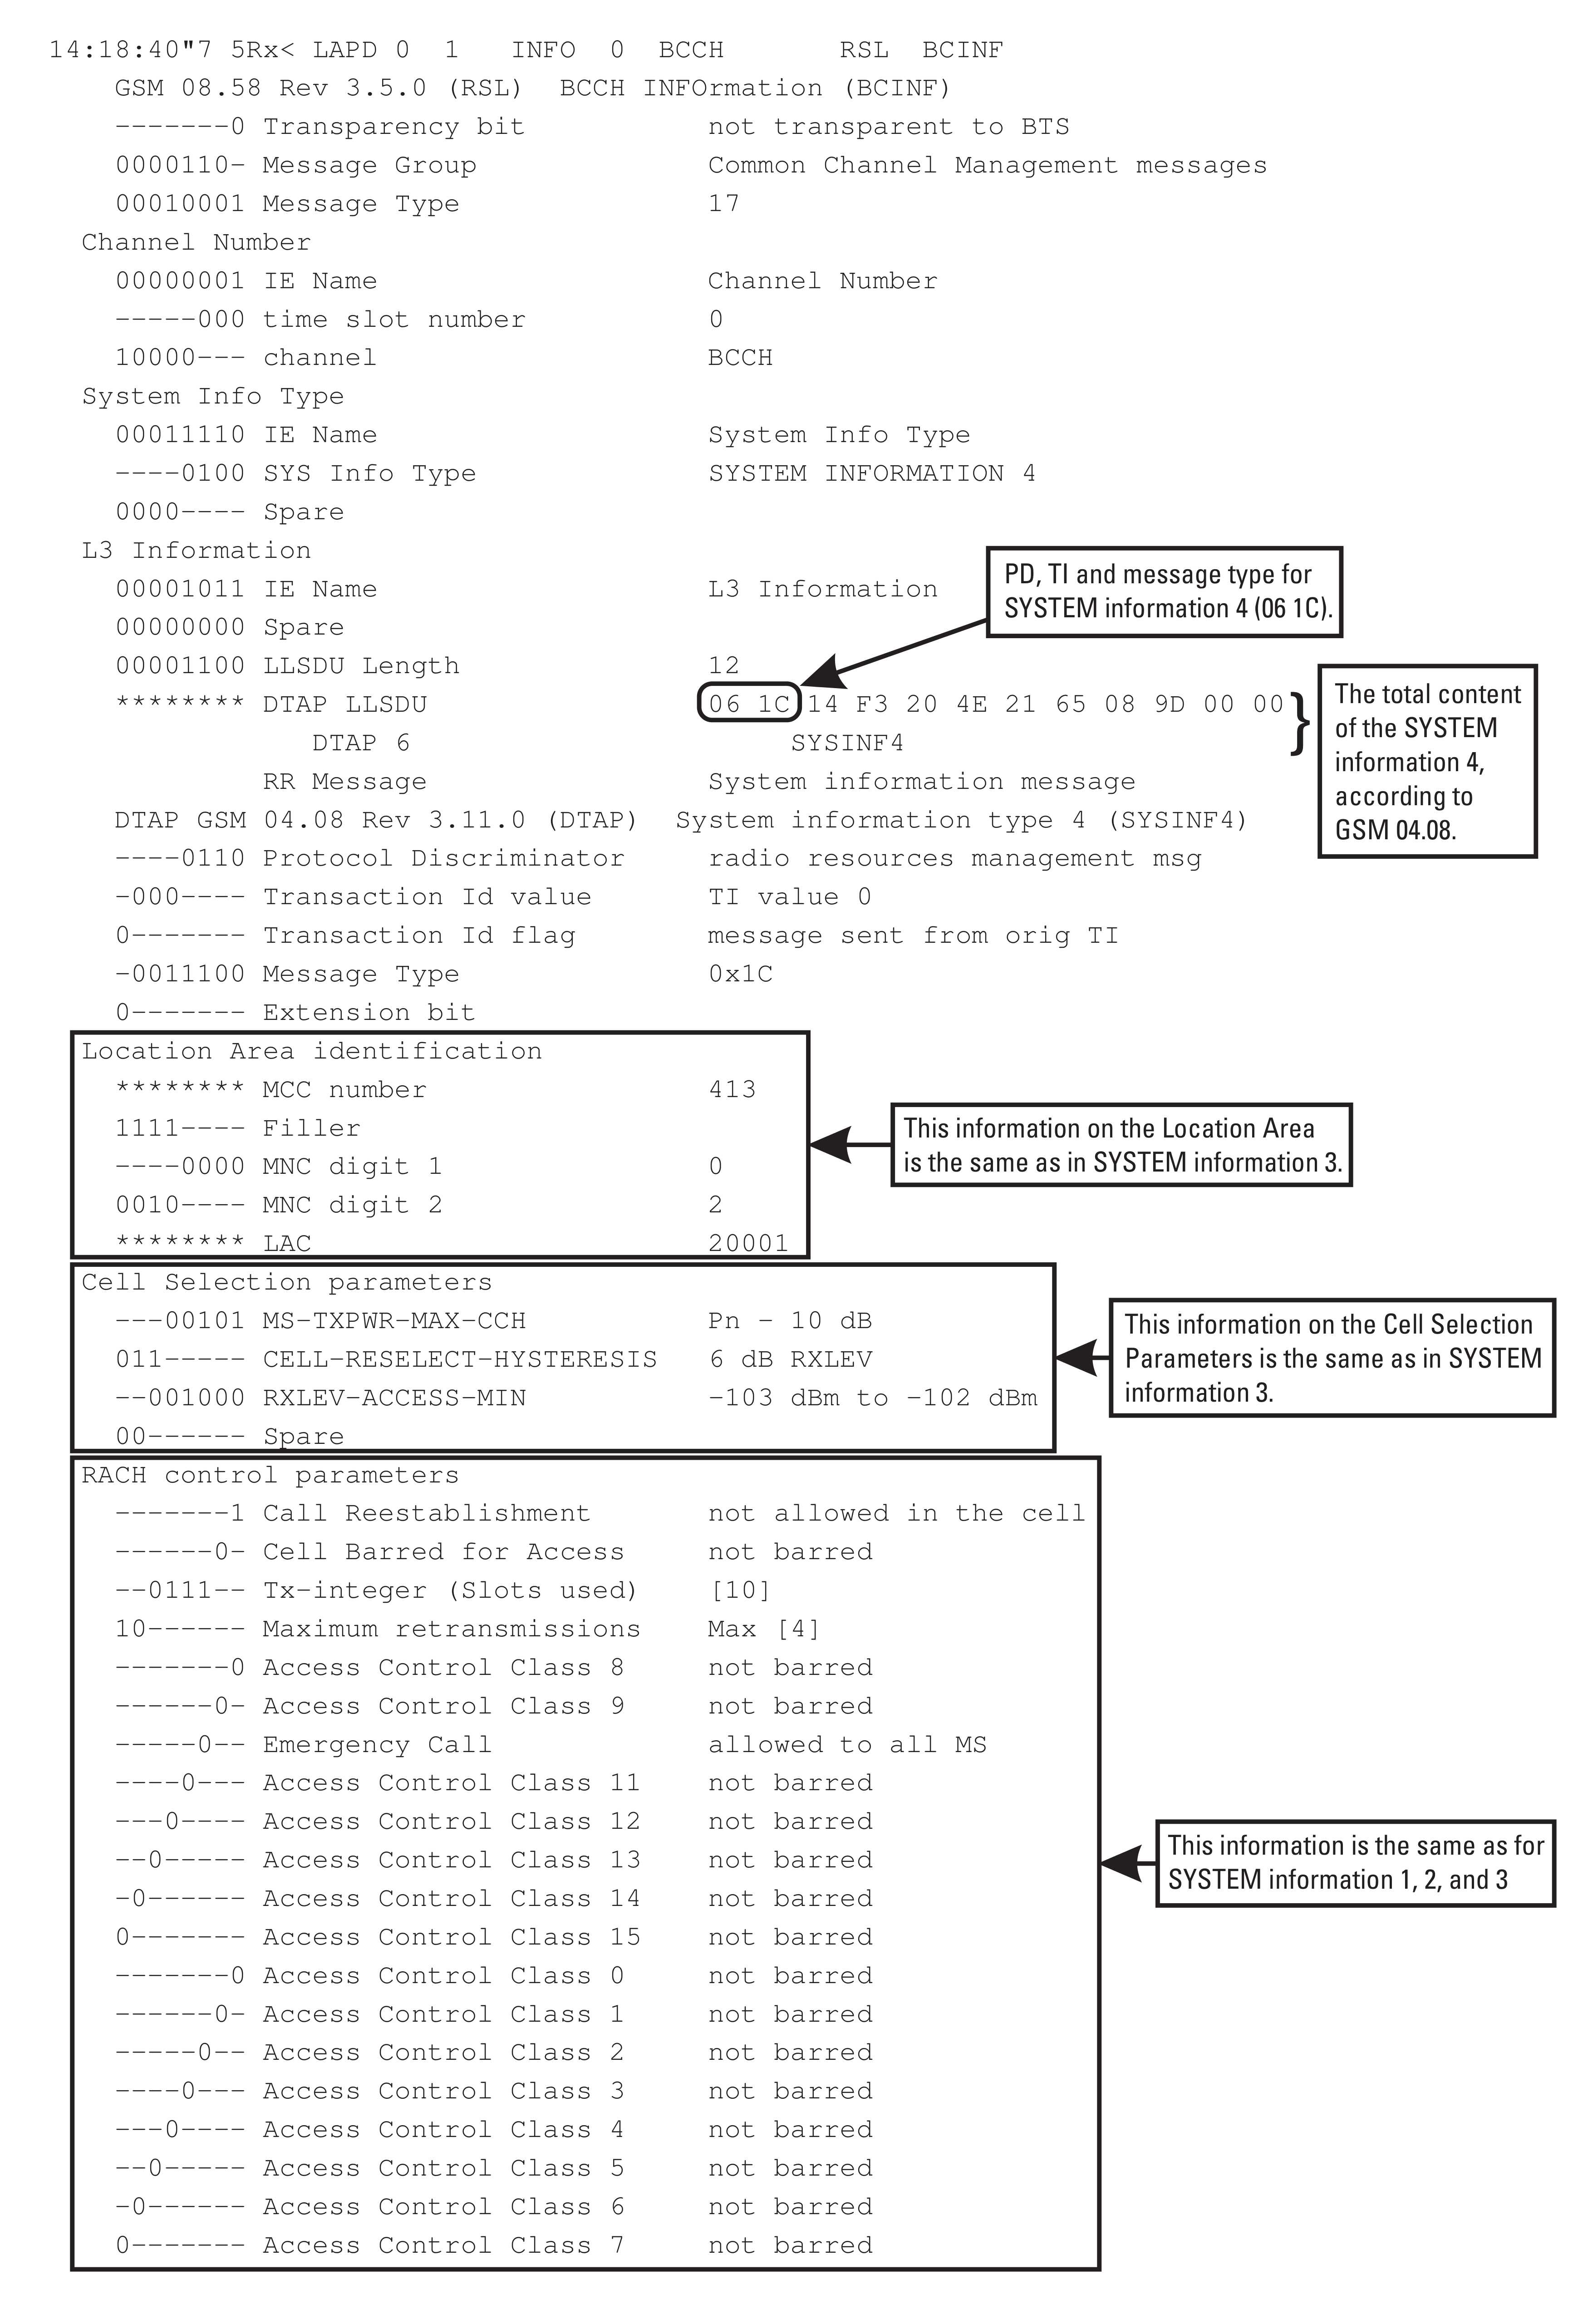
\includegraphics[width=.9\textwidth]{../Images/sysinfo4}
\caption{System Information 4 Message}
\end{figure}
\chapter{Evaluation Data}
\section{Rx and LAC Change Test}
\label{sec_lac_change_test}
The following table contains the four configuration that have been used to replace real base stations with the IMSI catcher.
\begin{center}
\begin{tabular}{lllll}
\toprule
			&T-Mobile		&O2				&E-Plus			&Vodafone\\
\midrule
ARFCN		&50				&2				&978			&695	\\
ShortName	&T-Mobile		&Vodafone		&E-Plus			&O2		\\
MCC			&262			&262			&262			&505	\\
MNC			&01				&02				&03				&07		\\
LAC			&21010			&793			&588			&50945	\\
Cell ID		&1				&2				&3				&4		\\
Neighbours	&-				&1,2,3			&695, 20		&10, 20, 30\\
\bottomrule
\end{tabular}
\end{center}
\section{Long Term Test}
\label{sec:long_term_test}
The folliwing tables contain the configurations that have been used throughout the long term test period.
The configurations have been used in the order they appear in the tables.
\begin{center}
\begin{tabular}{lllll}
\toprule
			&Conf. 1		&Conf. 2		&Conf. 3		&Conf. 4\\
\midrule
ARFCN		&50				&2				&978			&695	\\
ShortName	&T-Mobile		&Vodafone		&E-Plus			&O2		\\
MCC			&262			&262			&262			&505	\\
MNC			&01				&02				&03				&07		\\
LAC			&21010			&793			&588			&50945	\\
Cell ID		&1				&2				&3				&4		\\
Neighbours	&-				&1,2,3			&695, 20		&10, 20, 30\\
\bottomrule
\end{tabular}\\
\vspace{1cm}
\begin{tabular}{lllll}
\toprule
			&Conf. 5		&Conf. 6		&Conf. 7		&Conf. 8\\
\midrule
ARFCN		&50				&2				&978			&695	\\
ShortName	&T-Mobile		&Vodafone		&E-Plus			&O2		\\
MCC			&262			&262			&262			&505	\\
MNC			&01				&02				&03				&07		\\
LAC			&21010			&793			&588			&50945	\\
Cell ID		&1				&2				&3				&4		\\
Neighbours	&-				&1,2,3			&695, 20		&10, 20, 30\\
\bottomrule
\end{tabular}\\
\vspace{1cm}
\begin{tabular}{lllll}
\toprule
			&Conf. 9		&Conf. 10		&Conf. 11		&Conf. 12\\
\midrule
ARFCN		&50				&2				&978			&695	\\
ShortName	&T-Mobile		&Vodafone		&E-Plus			&O2		\\
MCC			&262			&262			&262			&505	\\
MNC			&01				&02				&03				&07		\\
LAC			&21010			&793			&588			&50945	\\
Cell ID		&1				&2				&3				&4		\\
Neighbours	&-				&1,2,3			&695, 20		&10, 20, 30\\
\bottomrule
\end{tabular}
\end{center}